\section{Misura della caratteristica corrente-tensione di un diodo}
In questa sezione abbiamo sostituito la resistenza nel circuito utilizzato in precedenza con un diodo. Esso è un elemento circuitale non lineare la cui funzione è quella di permettere alla corrente elettrica di fluire in un verso e di bloccarla quasi totalmente nell'altro.
Abbiamo proceduto variando la tensione di alimentazione del circuito, misurando la differenza di potenziale ai capi del diodo e la corrente che lo attraversava.
Nonostante la Legge di Shockley descriva l'andamento della corrente con una relazione esponenziale, nella realtà si usa definire una tensione di soglia, $V_{soglia}$, oltre la quale il diodo è considerato in conduzione.
In primis abbiamo verificato la legge sopra citata attraverso un fit esponenziale, in cui l'unico parametro era $I_{0}$, in quanto gli altri erano costanti o termini noti.
Di seguito è riportato il fit esponenziale

\begin{figure}[H]
    \centering
    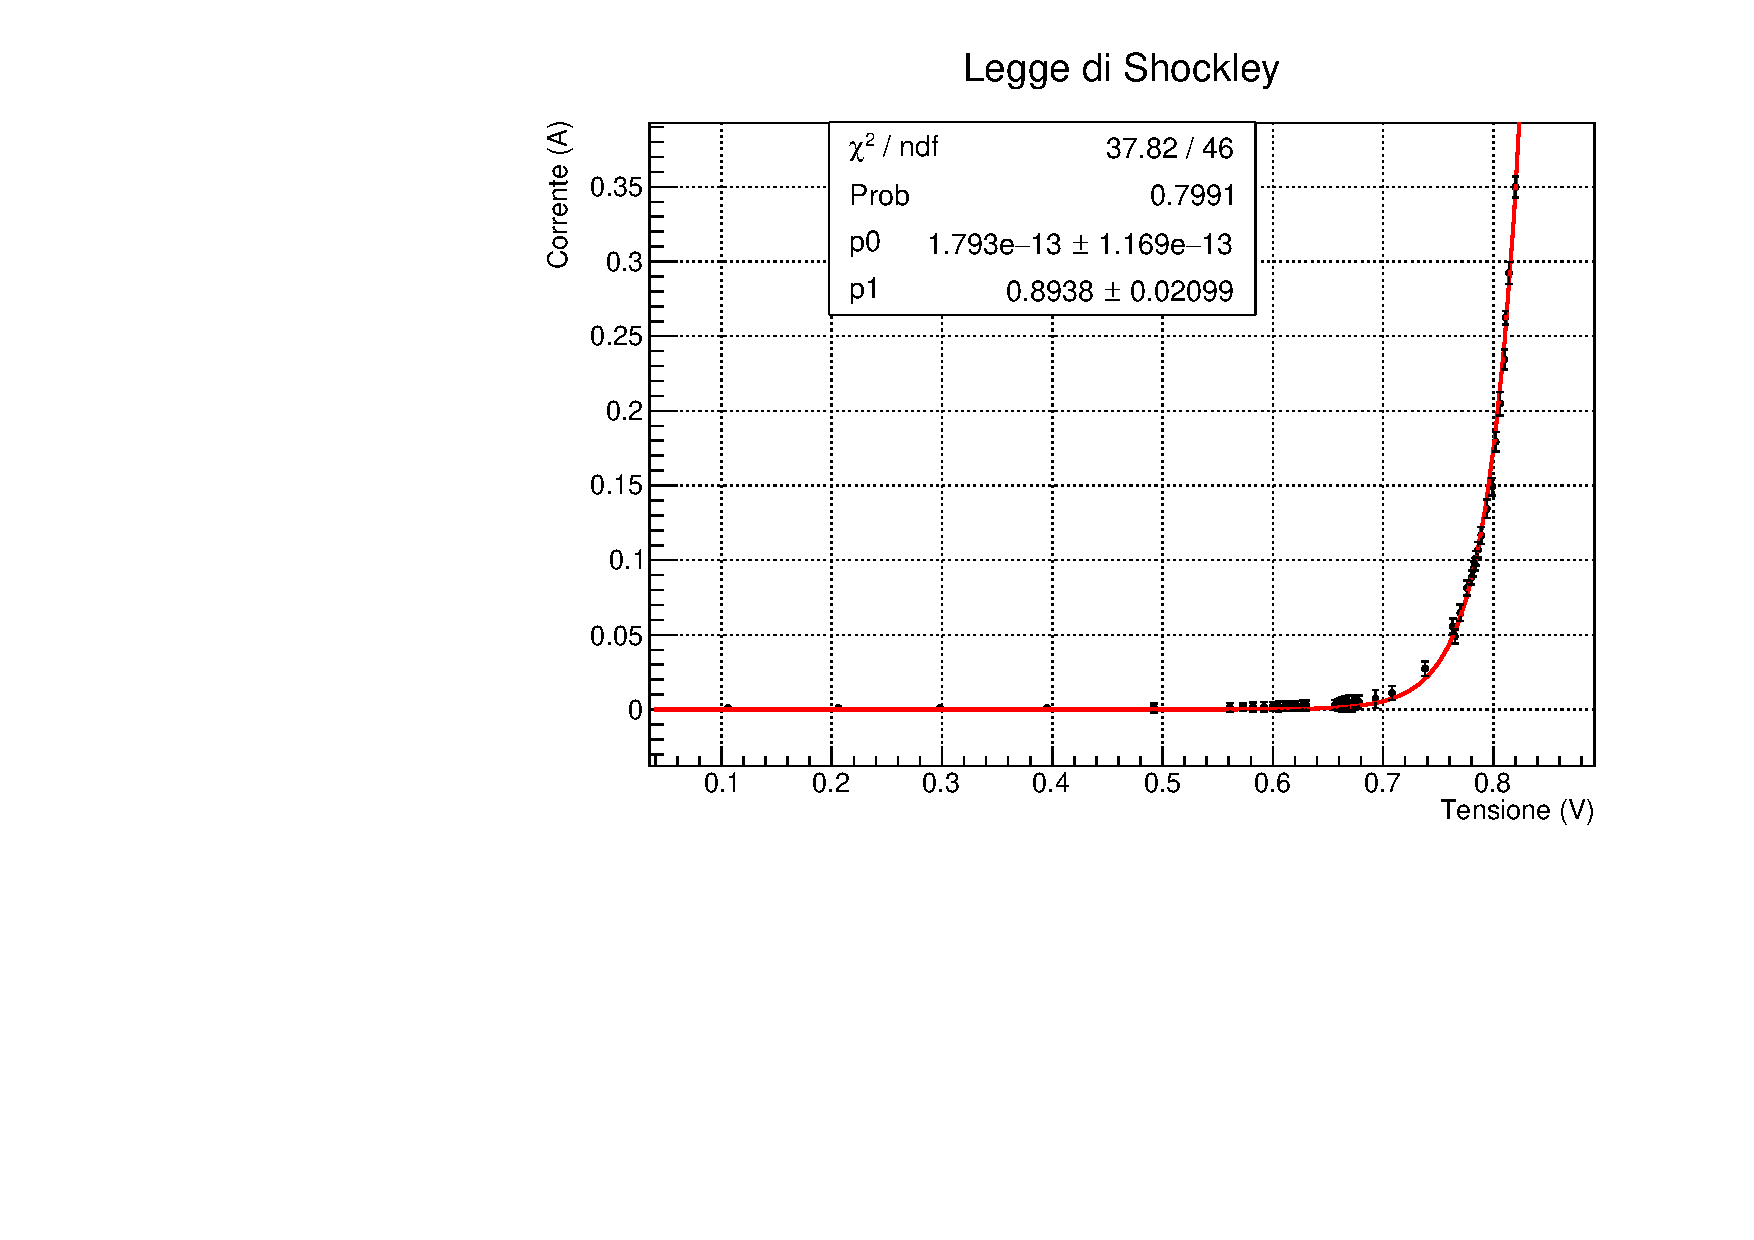
\includegraphics[scale=.5]{Immagini/diodo2.pdf}
    \caption{Fit con la legge di Shockley}
\end{figure}
In secondo luogo abbiamo individuato la $V_{soglia}$, fittando i dati con una retta, partendo dal range superiore delletensioni, fino a raggiungere un $\chi ^{2}$ ridotto di circa 1. Trovando l'intercetta di questaretta con l'asse \textit{x}, abbiamo ricavato $V_{soglia}$. Inoltre il parametro $p_0$ indica la corrente di saturazione che risulta essere dell'ordine del $10^{-13}$ come previsto dal modello teorico, mentre il parametro $p_1$ esprime il valore del rapporto $\frac{1}{g}$ dove $g$ è una costante che dipende dal materiale componente il diodo, pari circa a $1$ per diodi in germanio mentre circa $2$ per diodi in silicio. Da questo dato ricaviamo che $g\approx 1$ per cui l'ipotesi che il diodo sia composto da germanio risulta essere giustificata.
Di seguito è riportato il grafico con il fit della retta:

\begin{figure}[h!]
    \centering
    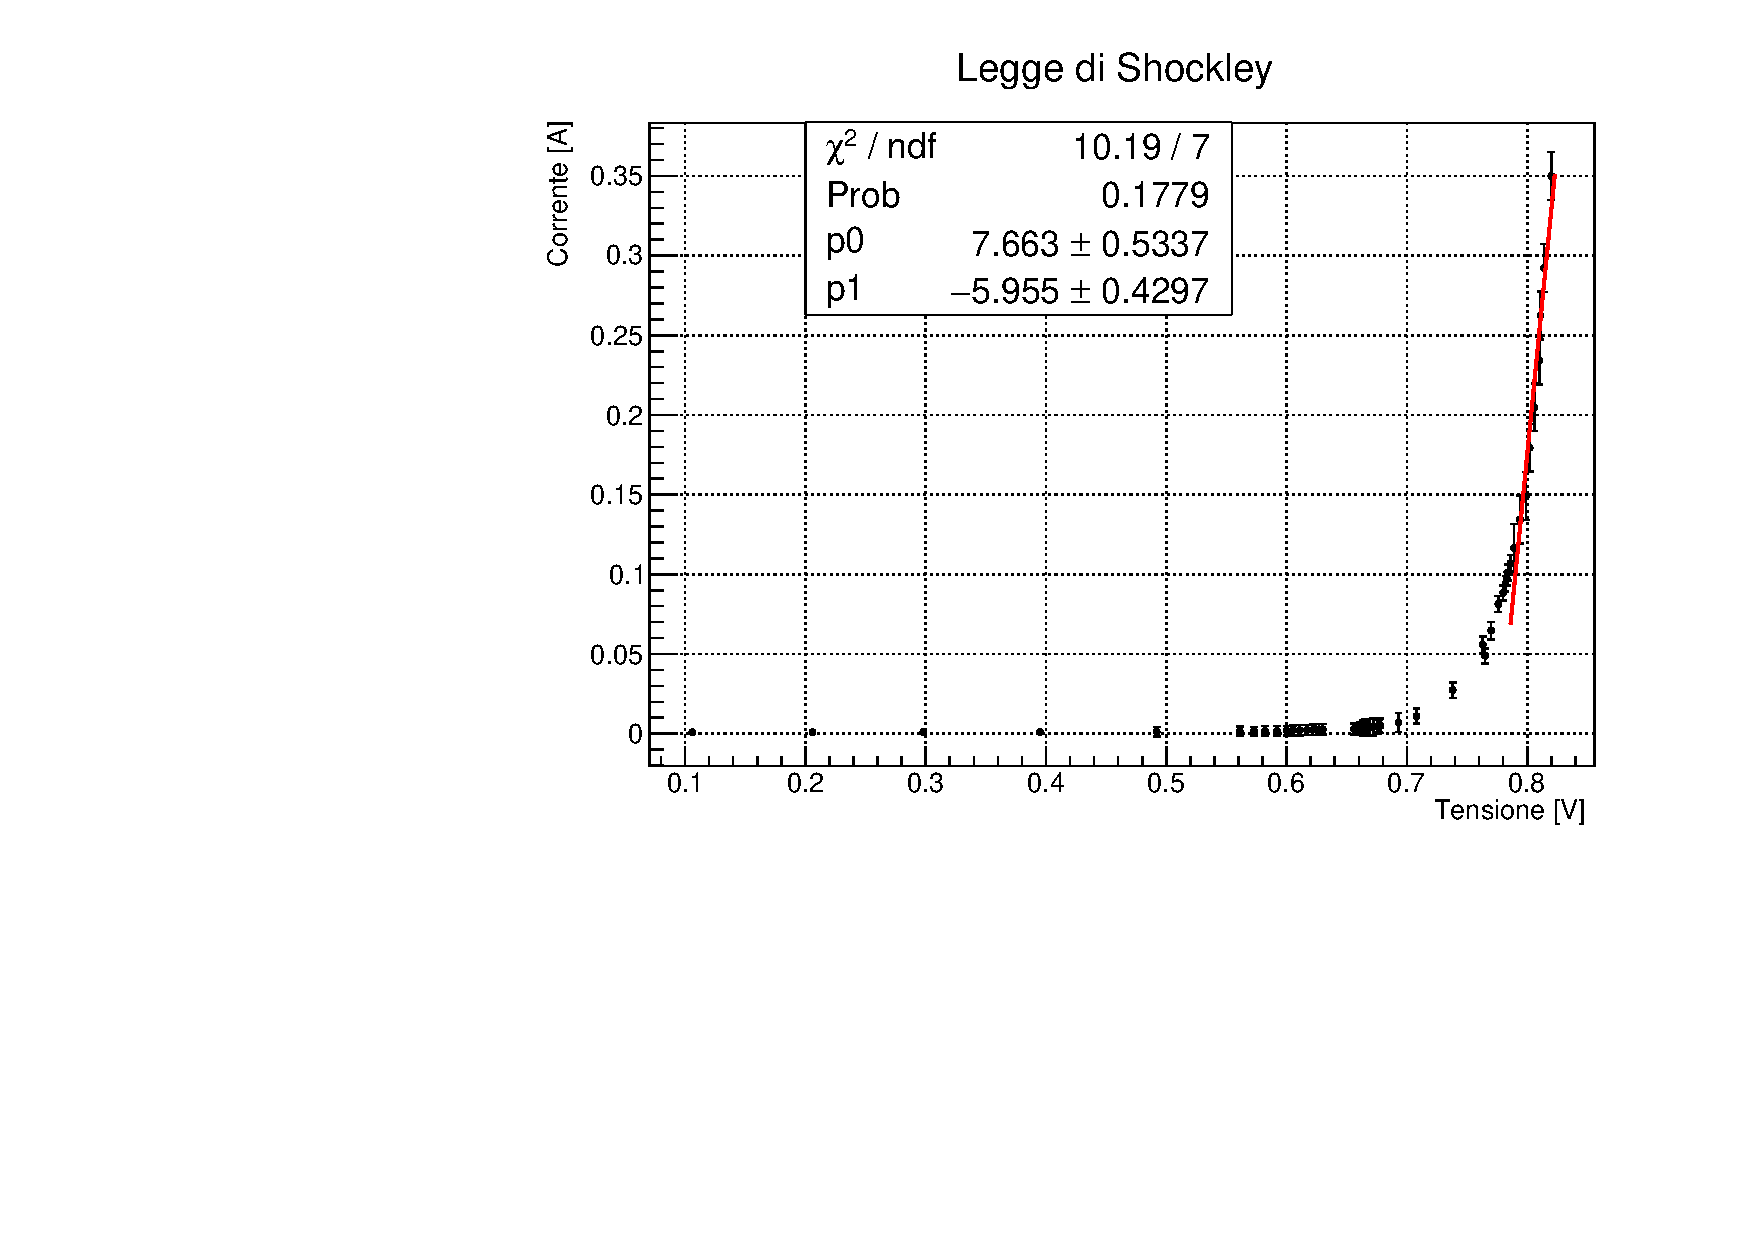
\includegraphics[scale=.5]{Immagini/diodo_soglia2.pdf}
    \caption{Fit con il diodo in conduzione da cui si ricava $V_{\text{soglia}}$ che corrisponde con il parametro $P_0$}
    \label{fig:my_label}
\end{figure}